\chapter{ARM Cortex-M4 Assembly Fundamentals}
\section*{Learning Objectives}
After completing this experiment, you will be able to:
\begin{itemize}[nosep]
  \item Identify the main components of the ARM Cortex-M4 architecture, including general-purpose registers, stack pointer, link register, program counter, and program status register (xPSR).
  \item Write, assemble, and debug a minimal ARM assembly program containing a vector table and \texttt{Reset\_Handler}.
  \item Use core data-processing, shift/rotate, and compare/test instructions to manipulate register data.
  \item Apply conditional execution and branching using condition codes (\texttt{EQ}, \texttt{NE}, \texttt{GT}, \texttt{LT}, etc.).
  \item Debug assembly programs in \keil\ using breakpoints, single-stepping, and register/memory inspection to analyze instruction effects.
\end{itemize}

\section*{Experiment Overview}
This experiment introduces the fundamentals of ARM Cortex-M4 assembly programming and the structure of a minimal embedded program. 
You will explore the processor's register set, status flags, and memory map, and learn how to write and debug low-level code that manipulates data and controls program flow.

\noindent In this experiment, you will:
\begin{itemize}[nosep]
  \item Examine the Cortex-M4 register architecture and understand how flags in the xPSR reflect instruction results.
  \item Build and assemble a minimal startup image with a vector table and \texttt{Reset\_Handler}.
  \item Practice data-processing and control-flow instructions, observing how they affect registers and flags.
  \item Use the \keil\ debugger to single-step through instructions and inspect register and memory changes.
\end{itemize}

By the end of this lab, you will understand the core building blocks of ARM assembly programming, from program structure and instruction execution to debugging at the register level.

\newpage
\etocsetnexttocdepth{subsubsection}
\localtableofcontents
\bigskip
\newpage
\section{Theoretical Background}
\subsection{Cortex-M4 Architecture}
\subsubsection{Registers Overview}
The Cortex-M4 architecture includes a set of general-purpose registers (R0-R12), a stack pointer (SP), a link register (LR), a program counter (PC), and a program status register (xPSR), all of which are 32-bit registers. The general-purpose registers are used for data manipulation and temporary storage during program execution. The SP is used to manage the call stack, while the LR holds the return address for function calls. The PC points to the next instruction to be executed, and the xPSR contains flags and status information about the processor state.
\paragraph{Program Status Register (xPSR)}
holds the current state of the processor, including condition flags (Negative, Zero, Carry, Overflow), interrupt status, and execution state. These flags are updated based on the results of arithmetic and logical operations, allowing for conditional branching and decision-making in programs.

\subsubsection{Memory Mapping}
The Cortex-M4 uses a flat memory model, where all memory locations are accessible through a single address space. This model simplifies programming and allows for efficient access to data and instructions. The memory is divided into several regions, including code memory (for storing instructions), data memory (for storing variables), and peripheral memory (for interfacing with hardware components). The architecture supports both little-endian and big-endian data formats, with little-endian being the default.
\begin{table}[H]
\centering
\caption{Cortex-M4 Memory Regions (ARMv7-M)}
\begin{tabularx}{\linewidth}{@{}p{0.20\linewidth}p{0.30\linewidth}X@{}}
\toprule
\textbf{Region} & \textbf{Address Range} & \textbf{Description} \\
\midrule
Code            & \texttt{0x00000000}--\texttt{0x1FFFFFFF} & Flash memory for program code \\[0.5ex]
SRAM            & \texttt{0x20000000}--\texttt{0x3FFFFFFF} & On-chip static RAM for data \\[0.5ex]
Peripheral      & \texttt{0x40000000}--\texttt{0x5FFFFFFF} & Memory-mapped peripheral registers \\[0.5ex]
External RAM    & \texttt{0x60000000}--\texttt{0x9FFFFFFF} & External RAM (if implemented) \\[0.5ex]
External Device & \texttt{0xA0000000}--\texttt{0xDFFFFFFF} & External devices/memory (if implemented) \\[0.5ex]
Private Peripheral Bus & \texttt{0xE0000000}--\texttt{0xE00FFFFF} & Cortex-M4 internal peripherals  (NVIC, SysTick, MPU, SCB)\\
System          & \texttt{0xE0100000}--\texttt{0xFFFFFFFF} & System region (reserved/system-level) \\
\bottomrule
\end{tabularx}
\end{table}


\subsection{Assembly Language Basics}

Assembly language is a low-level programming language that provides a direct correspondence between human-readable instructions and the machine code executed by the processor. Each instruction encodes a specific operation, such as moving data, performing arithmetic or logic, or altering control flow. Because it maps so closely to hardware, assembly allows precise control of system resources and is commonly used in performance-critical routines or when direct access to hardware is required.

Assembly programs are typically composed of three main elements: \emph{instructions}, \emph{directives}, and \emph{labels}.

\paragraph{Instructions}  
Instructions are the executable commands that the CPU carries out. Examples include data movement (\texttt{MOV}), arithmetic (\texttt{ADD}, \texttt{SUB}), logical operations (\texttt{AND}, \texttt{ORR}), and control flow (\texttt{B}, \texttt{BL}). Each instruction directly translates to one or more machine code opcodes and determines the actual behavior of the program.

\paragraph{Directives}  
Directives are commands to the assembler that guide how source code is translated into machine code but do not generate instructions themselves. Common examples include \texttt{AREA} (define a code or data section), \texttt{ALIGN} (align data to memory boundaries), \texttt{DCD} (allocate and initialize a word of storage), and \texttt{EXPORT} (export a symbol for linking). Directives organize program layout, control memory allocation, and manage symbol visibility.

\paragraph{Labels}  
Labels are symbolic names that mark specific locations in code or data. They act as targets for jumps and branches or as references for data access. Labels improve program readability and maintainability by avoiding hard-coded addresses. For instance, a label like \texttt{loop\_start} can be used as the destination of a branch instruction, and the assembler automatically computes the correct relative address.
\subsubsection{Instruction Set Overview}
The ARM Cortex-M4 instruction set is a subset of the ARMv7-M architecture, designed for efficient execution in embedded systems. It includes a variety of instructions for data processing, memory access, and control flow. Key categories of instructions include:
\hfill
\begin{itemize}[nosep]
    \item \textbf{Data Processing Instructions}: These include arithmetic operations (e.g., \texttt{ADD}, \texttt{SUB}), logical operations (e.g., \texttt{AND}, \texttt{ORR}), and data movement instructions (e.g., \texttt{MOV}, \texttt{MVN}).
    \item \textbf{Load and Store Instructions}: Instructions like \texttt{LDR} (load register) and \texttt{STR} (store register) are used to transfer data between registers and memory.
    \item \textbf{Branch Instructions}: Control flow is managed using branch instructions such as \texttt{B} (branch), \texttt{BL} (branch with link), and conditional branches like \texttt{BEQ} (branch if equal).
    \item \textbf{Special Instructions}: These include instructions for system control, such as \texttt{NOP} (no operation), \texttt{WFI} (wait for interrupt), and instructions for manipulating the stack and handling exceptions.
\end{itemize}
\subsubsection{General Instruction Format}

Assembly source lines generally follow this shape:

\[
\texttt{[label]} \quad \texttt{OPCODE\{<cond>\}\{S\}} \quad \texttt{operands} \quad \texttt{\color{lightgray}; comment}
\]

where curly braces \texttt{\{\}} denote optional components, and:
\begin{itemize}[nosep]
  \item \texttt{label}: optional symbolic name marking the current address.
  \item \texttt{OPCODE}: instruction mnemonic (e.g., \texttt{ADD}, \texttt{MOV}, \texttt{B}).
  \item \texttt{<cond>}: optional condition code (e.g., \texttt{EQ}, \texttt{NE}, \texttt{LT}, \texttt{GE}) that predicates execution.
  \item \texttt{S}: optional suffix indicating whether to update the condition flags (e.g., \texttt{ADDS}).
  \item \texttt{operands}: registers, immediates, or memory operands (e.g., \texttt{R0, R1, \#1} or \texttt{[R2]}).
  \item Anything after a semicolon (\texttt{;}) is a comment ignored by the assembler.
\end{itemize}

\begin{lstlisting}[caption={Instruction format example}]
loop_start   ADDS   R0, R0, #1      ; R0 = R0 + 1, update flags (N,Z,C,V)
\end{lstlisting}


\subsection{Basic Program Template (Boilerplate)}

The minimal skeleton below shows a valid vector table in a \texttt{READONLY} \texttt{RESET} area, a \texttt{READWRITE} data area for variables, and a code area with the \texttt{Reset\_Handler} entry point.

\begin{lstlisting}[caption={Cortex-M4 boilerplate with READWRITE data}]
        AREA    RESET, CODE, READONLY     ; Vector table lives in read-only code
        EXPORT  __Vectors                 ; Make symbol visible to the linker
__Vectors
        DCD     0x20001000                ; Initial SP value (top of stack in SRAM)
        DCD     Reset_Handler             ; Reset vector: entry address
        ALIGN        
        ; -------------------- Read-Write Data --------------------
        AREA    M_DATA, DATA, READWRITE   ; Variables go here (RAM)
        EXPORT  COUNT                     ; Export if referenced by other modules
COUNT   DCD     0                         ; Initialized RW variable (word)
BUF     SPACE   16                        ; Uninitialized RW buffer (16 bytes)
        ALIGN        
        ; -------------------- Application Code -------------------
        AREA    MYCODE, CODE, READONLY
        ENTRY
        EXPORT  Reset_Handler
Reset_Handler
        ; Example: COUNT++ and store to BUF[0]
        LDR     R0, =COUNT                ; R0 <- &COUNT
        LDR     R1, [R0]                  ; R1 <- COUNT
        ADDS    R1, R1, #1                ; R1 = R1 + 1 (update flags)
        STR     R1, [R0]                  ; COUNT <- R1        
        LDR     R2, =BUF                  ; R2 <- &BUF
        STRB    R1, [R2]                  ; BUF[0] <- (low byte of R1)
STOP    B       STOP                      ; Stay here forever
        END
\end{lstlisting}

\paragraph{What each directive does}
\begin{itemize}[nosep]
  \item \texttt{AREA <name>, CODE|DATA, READONLY|READWRITE}:
        defines a section. Put the vector table and program text in \texttt{CODE, READONLY};
        put variables in \texttt{DATA, READWRITE}.
  \item \texttt{EXPORT <symbol>}: makes a label visible to the linker/other modules.
  \item \texttt{DCD, DCW, DCB <values>}: allocate and initialize words, halfwords, or bytes.
  \item \texttt{SPACE <n>}: reserve \textit{n} bytes of uninitialized storage in RAM.
  \item \texttt{ALIGN}: align to a suitable boundary (commonly 4 bytes for words).
  \item \texttt{ENTRY}: mark the entry point of the image for the toolchain.
  \item \texttt{END}: end of source file.
\end{itemize}

\paragraph{Notes}
\begin{itemize}[nosep]
    \item The first two words in \texttt{\_\_Vectors} must be the initial stack pointer value and the address of \texttt{Reset\_Handler}.
    \item The assembler/linker places sections in appropriate memory regions based on the target device and linker script.
    \item Labels must start at the beginning of the line (no indentation), while instructions and directives should be indented for proper assembly.
    \item Variables in \texttt{READWRITE} areas are initialized to zero by default. While you can specify initial values using directives like \texttt{DCD}, the linker will place these in flash and copy them to RAM during startup, or they may be zeroed out during RAM initialization.
\end{itemize}

\newpage
\section{Procedure}
\subsection{Setting Up the Keil uVision5 Environment}
Make sure you have the \keil\ IDE installed on your computer. If not, download and install it from the official Keil website (\url{https://www.keil.com/demo/eval/arm.htm}). 
\subsubsection{Creating a New Project}
\begin{enumerate}[nosep]
    \item Open \keil\ and create a new project:
    \begin{itemize}[nosep]
        \item Go to \texttt{Project > New uVision Project...}
        \item Choose a directory and name for your project (e.g., \texttt{Exp01\_ARM\_Assembly}).
    \end{itemize}
    \item Select the target device:
    \begin{itemize}[nosep]
        \item In the "Select Device for Target" dialog, choose ARM Cortex-M4 (ARMCM4) as we will be using it only for simulation.
        \item Click "OK" to confirm.
    \end{itemize}
    \item Configure project settings:
    \begin{itemize}[nosep]
        \item Go to \texttt{Project > Options for Target 'Target 1'...}
        \item Under the "Debug" tab, select "Use Simulator" as the debug driver.
    \end{itemize}
    \item Add a new assembly file to the project:
    \begin{itemize}[nosep]
        \item Right-click on "Source Group 1" in the Project window and select \texttt{Add New Item to Group 'Source Group 1'...}
        \item In the "Add New Item" dialog, select "Assembly File" from the list.
        \item Name the file (e.g., \texttt{main.s}) and click "Add".
    \end{itemize}
    \item Build the project:
    \begin{itemize}[nosep]
        \item Click on the "Build" button (or go to \texttt{Project > Build Target}), or use the shortcut \texttt{F7}.
        \item Check the "Output" window for any errors or warnings. If there are errors, fix them in your assembly code and rebuild.
        \item Once the build is successful, you should see a message indicating that the build was completed without errors.
    \end{itemize}
    \item Start a debugging session:
    \item Click on the "Debug" button (or go to \texttt{Debug > Start/Stop Debug Session}), or use the shortcut \texttt{Ctrl + F5}.
\end{enumerate}
\clearpage
\subsubsection{Debugging and Running the Program}
\begin{figure}[H]
    \centering
    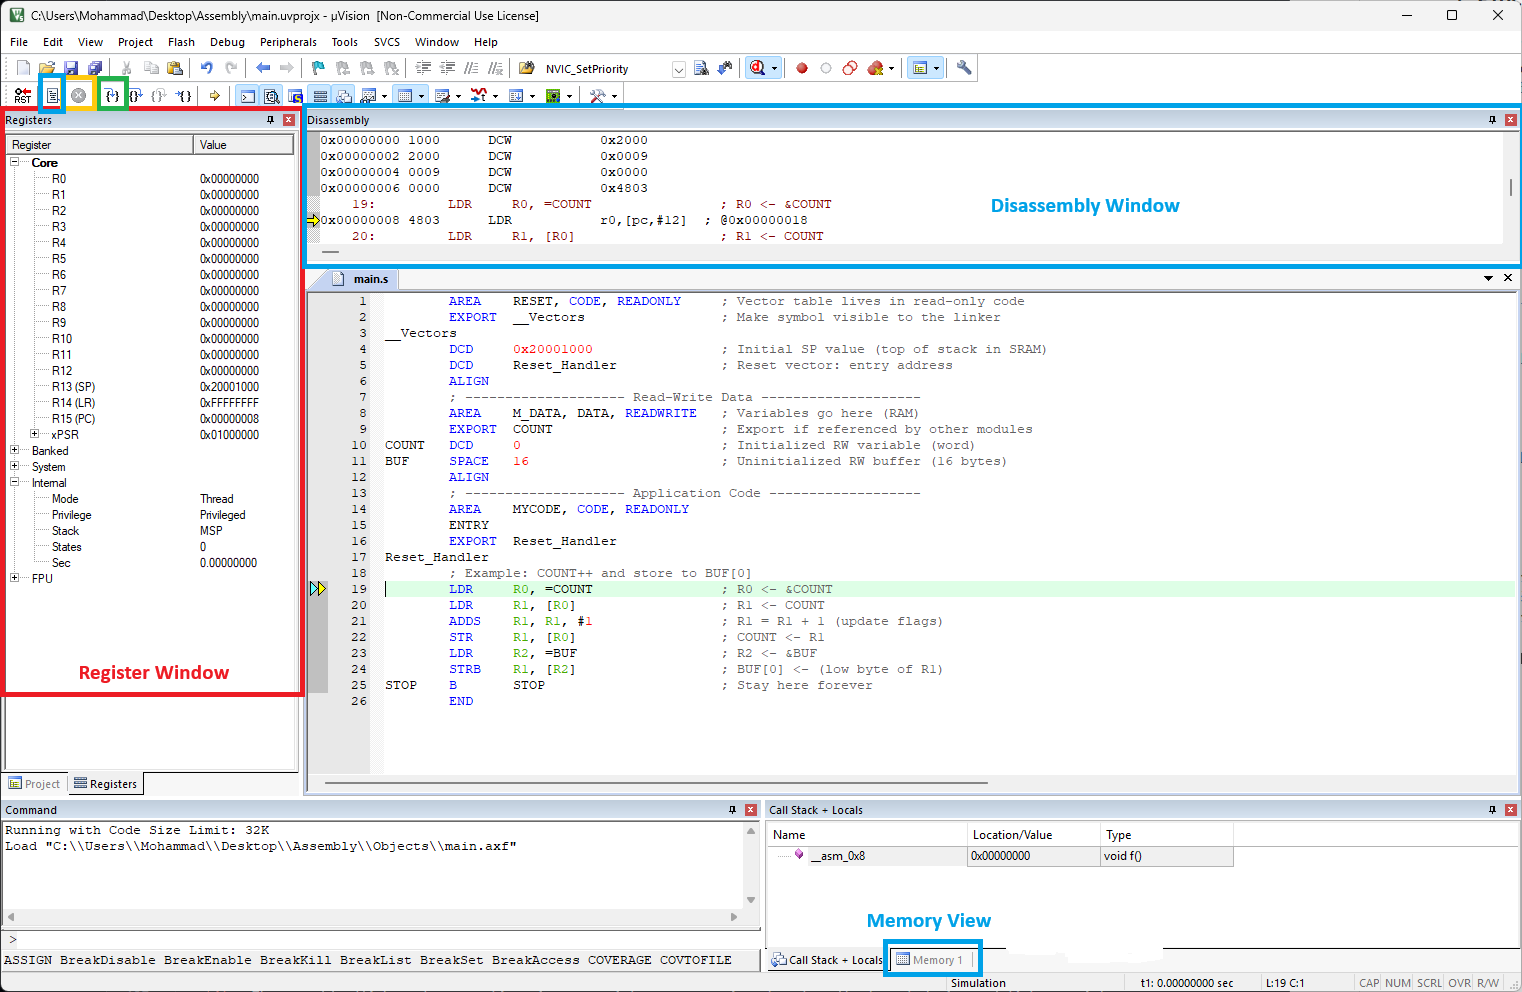
\includegraphics[width=\textwidth]{resources/keil_debug.png}
    \caption{Keil uVision5 Debugging Interface}
    \label{fig:keil_debug}
\end{figure}
Figure \ref{fig:keil_debug} shows the Keil uVision5 debugging interface. You can run and debug your assembly program using two main approaches:
\begin{enumerate}[nosep]
    \item \textbf{Step by Step Execution}:
    \begin{itemize}[nosep]
        \item Use the "Step" button (or press \texttt{F11}) marked in green in Figure \ref{fig:keil_debug} to execute your program one instruction at a time.
        \item Observe the changes in the registers and memory as you step through each instruction.
    \end{itemize}
    \item \textbf{Run the entire program}:
    \begin{itemize}[nosep]
        \item Use the "Run" button (or press \texttt{F5}) marked in blue in Figure \ref{fig:keil_debug} to execute your program continuously until it hits a breakpoint or completes execution.
        \item After running, you must stop the execution using the "Stop" button marked in yellow in Figure \ref{fig:keil_debug}.
        \item Check the final values in the registers and memory to verify the program's behavior.
    \end{itemize}
\end{enumerate}
\newpage
\subsection{Examples}
\subsubsection{Example 1: Simple Arithmetic Operations and Flag Manipulation}
The following example demonstrates basic arithmetic operations, flag manipulation.
\lstinputlisting[caption={Example 1: Simple Arithmetic Operations and Flag Manipulation}]{snippets/assembly/exp1/example1.asm}
